%bib=bibtex
\documentclass[a4paper]{article}

\usepackage[utf8]{inputenc}
\usepackage{ifthen,etoolbox}
\usepackage[british]{babel} %languages nicely, with proper date format courtesy of [british]
\usepackage{csquotes} %helps to quotes nicely
%\usepackage{float} %for control over figure positioning

\usepackage{hyperref} %hyperlinks contents and references
\usepackage{graphicx} %required for image manipulation
\usepackage[a4paper, top=25mm,bottom=25mm,left=25mm,right=25mm]{geometry} %allows manipulation of page structure
\usepackage{cite} %BibTeX bibliography manager
\usepackage{amsmath, amssymb} %adds many fancy maths symbols and things

%\usepackage{epstopdf}
%\usepackage{url}
%\usepackage{setspace}
%\usepackage{titlesec}

\graphicspath{{../../plots/}}

%\usepackage{abstract}
%\addto\captionsenglish{\renewcommand{\abstractname}{}}
%\addto\captionsenglish{\renewcommand{\absnamepos}{empty}}

\title{Analysis Note: Measurement of forward $W$ and $Z$ boson cross sections in $pp$ collisions at $\sqrt{s}=5 \; \rm{TeV}$}
\author{Laura Cairns}
\date{\today}

\begin{document}
\maketitle

\begin{abstract}
    \noindent 
    Measurements of electroweak boson production cross sections are presented for $pp$ collisions at centre of mass energy $\sqrt{s} = 5$ TeV. The data analysed was collected at the LHCb detector with an integrated luminosity of \input{results/lumi_value.tex}. Muon decay channels are studied within the kinematic region defined by pseudorapity $2.0 < \eta < 4.5$ and transverse momenta $p_T > 20$~GeV. The boson cross sections are found to be
    \input{results/Z_xsec_output.tex}
    \input{results/Wp_xsec_output.tex}
    \input{results/Wm_xsec_output.tex}
    where statistical uncertainties, and uncertainties due to trigger efficiency and luminosity are labelled. Ratios of these cross sections are also determined as 
    \input{results/WW_ratio_output.tex}
    \input{results/WZ_ratio_output.tex}
\end{abstract}


\section{Z Cross Section from 5TeV Experimental Data} \label{results}

The LHCb dataset used in this analysis has been taken at $\sqrt{s} = 5$ TeV. The dataset contains 5840 entries. The workflow of the code used to analyse this data is given in Section \ref{workflow}, with results given in Section \ref{results}, and plots given in Section \ref{Z histograms}.

\subsection{Integrated Luminosity} \label{lumi_val}
Integrated Luminosity $L$ assumed to have percentage uncertainty of 5.0\%.\\$L = 64.6 \pm 3.2 \; {\rm pb^{-1}}$\\

\subsection{Trigger Efficiency} \label{trigger_val}
Trigger Efficiency = $0.9957 \pm 0.0009$\\Trigger Efficiency Relative Uncertainty = $0.00086$\\

\subsection{Z Counts} \label{counts_val}
Counts in Fiducial Region = $3748 \pm 61 \; \rm counts$\\Counts Relative Uncertainty = $0.0163$\\

\subsection{Z Cross Section} \label{xsec_val}
\input{results/Z_xsec_output.tex}


\section{Workflow of Z Analysis} \label{workflow}

\subsection{Comparison of Experimental Data with Monte Carlo Simulation} \label{sec: Z MC comparison}
In the code \texttt{plot$\_$MC$\_$comparison.cpp}, histograms are plotted using ROOT, comparing a number of variables from the 5 TeV LHCb dataset to a Monte Carlo simulation of the experiment. The Monte Carlo simulation was created in \textit{Pythia} and has 338926 entries, which have been passed through detector reconstruction. Simulation data has been scaled to the experimental data in the histogram plots, with each plotted using 100 bins.
The variables compared are:
\begin{itemize}
  \item Transverse Momentum $p_T$, separately for both positive and negative muons
  \item Pseudorapidity $\eta$, separately for both positive and negative muons
  \item Azimuthal angle $\phi$, separately for both positive and negative muons
  \item Dimuon invariant mass $M_{\mu\mu}$, equivalent to the mass of the Z boson $m_Z$
\end{itemize}

Differences can be seen between the experimental and simulated data due to background in the experimental data, and inaccuracies in the simulation. These inaccuracies arise due to the leading order precision of \textit{Pythia} and limits on the precision to which the detector can be described. 
Comparing these plots tests the validity of using the simulation in determination of $W$ boson background.

See plots in Section \ref{Z histograms}.

\subsection{Luminosity Calculation} \label{sec: Z lumi}
The code \texttt{get$\_$luminosity.py} calculates the integrated luminosity $L$ as the sum of 38 entries, where each entry represents a fraction of the data collected in the 5 TeV run.
The error on luminosity is assumed to be 5$\%$.
Integrated luminosity and its error are output as a json file ``luminosity.json", with their values given in Section~\ref{lumi_val}.
 
\subsection{Trigger Efficiency Calculation} \label{sec: Z trigger efficiency}
The code \texttt{measure$\_$trigger$\_$eff.py} calculates the trigger efficiency $\varepsilon_{\rm trigger}$, which forms the dominant systematic error in Z cross section calculation. 
Events where the positive muon or negative muon trigger are counted in the fiducial region (see \ref{sec: Z xsec}), as well as the events where both muons trigger. 
By requiring that one muon triggers (the tag muon), then there is no bias on the other muon (the probe muon). Hence, the efficiency of the probe muon trigger can be calculated as:
\begin{equation}
{\varepsilon}_{{\rm probe \;  muon}} = \frac{{\rm number \; of \; events \; where \; both \; muons \; trigger}}{{\rm number \; of \; events \; where \; tag \; muon \; triggers}}.
\end{equation}

This gives the trigger efficiencies of the positive and negative muons $\varepsilon_{\mu^+}$ and $\varepsilon_{\mu^-}$ as
\begin{equation}
    \varepsilon_{\mu^+} = \frac{N_{\mu^- + \mu^+}}{N_{\mu^-}},
    \label{eq: mup_eff}
\end{equation}
\begin{equation}
    \varepsilon_{\mu^-} = \frac{N_{\mu^- + \mu^+}}{N_{\mu^+}},
    \label{eq: mum_eff}
\end{equation}
where $N$ represents the number of events where the indicated muon(s) triggers. These efficiencies are used in the determination of $W^+$ and $W^-$ cross sections respectively (see Section \ref{sec: W xsec}).
The trigger efficiency used in the $Z$ analysis is calculated as the efficiency of either muon causing a trigger to activate (TOS), given as
\begin{equation}
    \varepsilon_{\mu\mu} = \varepsilon_{\mu^+} + \varepsilon_{\mu^-} - \varepsilon_{\mu^+} \times \varepsilon_{\mu^-}.
    \label{eq: either eff}
\end{equation}
The relative uncertainty on each efficiency is determined using the binomial formula $\sqrt{\varepsilon(1-\varepsilon/N}$ where $N$ represents the sample size. In this analysis, $N$ is given as the number of $Z$ events in the fiducial region.
The trigger efficiencies and their relative uncertainties are output as a json file ``efficiencies.json", with the trigger efficiencies given in Section \ref{trigger_val}.

\subsection{Z Cross Section Calculation} \label{sec: Z xsec}
The code \texttt{measure$\_$xsec.py} calculates the integrated cross section of Z $\sigma_Z$.
The number of events in the fiducial region $N_{\rm fiducial}$ are counted. The fiducial region is comprised of the kinematic cuts:

\begin{itemize}
  \item $60 < M_{\mu\mu} < 120 \; {\rm GeV}$ 
  \item $p_T > 20 \; {\rm GeV}$ for both positive and negative muons
  \item $2.0 < \eta < 4.5$ for both positive and negative muons
\end{itemize}

$\sigma_Z$ is then calculated as
\begin{equation}
\sigma_Z = \frac{N_{\rm fiducial}}{L \times {\varepsilon_{\rm trigger}}},
\label{eq: Z_xsec}
\end{equation}
using the previously calculated values of integrated luminosity $L$ and trigger efficiency $\varepsilon_{\rm trigger}$, read in from their respective codes.

Errors are propagated through $\sigma_Z$ according to the equation,
\begin{equation}
    \alpha_\sigma = \sigma \sqrt{\left(\frac{\alpha_N}{N}\right)^2 + \left(\frac{\alpha_L}{L}\right)^2 + \left(\frac{\alpha_\varepsilon}{\varepsilon}\right)^2},
    \label{eq: xsec error}
\end{equation}
and given separately in the result as statistical error (from the number of counts), and errors due to efficiency and luminosity. Errors are separated according to the following equation, with the statistical error given as an example;
\begin{equation}
    \alpha_{\sigma {\rm stat}} = \frac{\alpha_N}{N}\sigma.
    \label{eq: xsec error separation}
\end{equation}
%Error analysis on $\sigma_Z$ is carried out using the relative uncertainties on the number of counts, trigger efficiency, and luminosity. Each of these uncertainties is given separately in the result, with the uncertainty on the number of counts representing the statistical error. 
The cross section is output to a json file ``Z$\_$xsec.output", and its value can be seen in Section \ref{xsec_val}, whilst the value of counts can be seen in Section \ref{counts_val}.


\section{W Boson Analysis} \label{sec: W boson}

\subsection{Plotting W Data} \label{sec: W plotting}

The $p_T$ distributions of $W \xrightarrow{} \mu \nu_\mu$ decays are plotted for both $W^+$ and $W^-$ in the program \texttt{plot$\_$W$\_$dist.cpp}. 
The $W$ signal is isolated by calculating the isolation; the sum of $p_T$ for all particles surrounding the muon in a cone satisfying
\begin{equation}
    \sqrt{\Delta\eta^2 + \Delta\phi^2} < 0.5.
    \label{eq: isolation}
\end{equation}
The inverse of transverse momentum $p_T^{-1}$ are plotted against this isolation, as shown for both $W^+$ and $W^-$ in the histograms below (Figure \ref{fig: LEGO}. These figures use the LEGO plotting option. An additional plot is provided of the COLZ plotting option for $W^+$ in Figure \ref{fig: COLZ}. %Figure from interim report, not created in current workflow (18.02.2021) 
The $W$ decay signal can be seen as a peak between $p_T^{-1}$ = 0.02 and 0.03 GeV$^{-1}$ at low values of isolation, shown prominently in the COLZ plot. The LEGO plots highlight the charged $\pi/K$ background, identified as the Gaussian peak at high $p_T^{-1}$.


\begin{figure*}[t]
\centering
\includegraphics[clip, trim = 0.3cm 0.3cm 1.7cm 1.3cm,width=0.49\textwidth]{W+_isolated_signal.pdf}
\includegraphics[clip, trim = 0.3cm 0.3cm 1.7cm 1.3cm,width=0.49\textwidth]{W-_isolated_signal.pdf} %\hspace{3mm}
\vspace{-4mm}
\caption{\small Histogram plots of inverse transverse momentum $p_T^{-1}$ against the log of the isolation for the $W \xrightarrow{} \mu \nu_\mu$ decay. $W^+$ and $W^-$ are shown left and right respectively Plotted using the LEGO option.}
\label{fig: LEGO}
\end{figure*}

\begin{figure}[!hb]
    \centering
    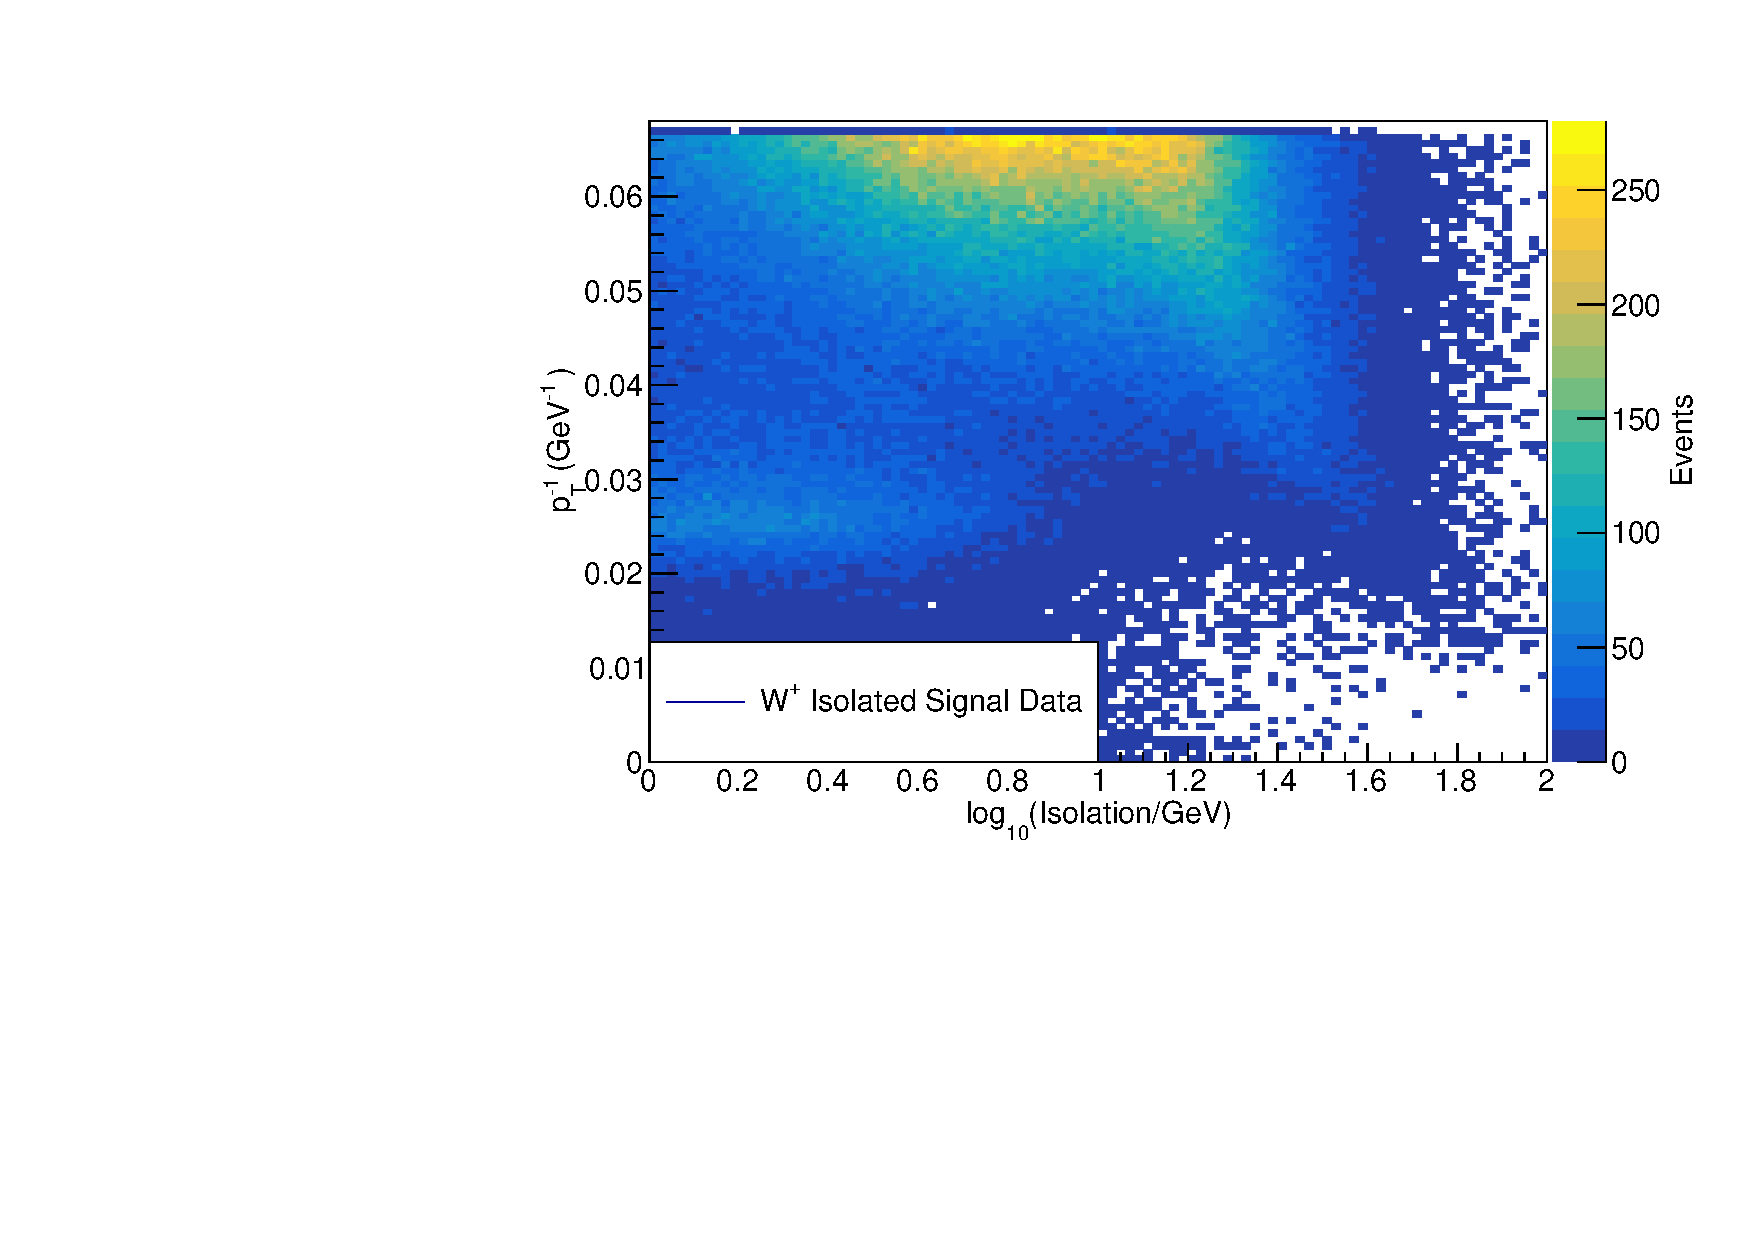
\includegraphics[clip, trim = 0cm 0cm 0.3cm 1.3cm, width=\textwidth]{../doc/measurement_doc/W+_isolated_signal_COLZ.pdf}
    \vspace{-4mm}
    \caption{\small COLZ plot of inverse transverse momentum $p_T^{-1}$ against the log of the isolation for the $W \xrightarrow{} \mu \nu_\mu$ decay for $W^+$.}
    \label{fig: COLZ} %Figure from interim report, not created in current workflow (18.02.2021)
\end{figure}


\subsection{W Background Analysis} \label{sec: W background}

The code \texttt{W$\_$background.cpp} plots and analyses the various background contributions to the $W^+$ and $W^-$ data.

The files used are:
\begin{itemize}
    \item Data: \texttt{5TeV$\_$2017$\_$32$\_$Down$\_$EW.root}
    \item Simulation of W signal: \texttt{5TeV$\_$2015$\_$24r1$\_$Down$\_$W$\_$Sim09d.root}
    \item Simulation of Z production: \texttt{5TeV$\_$2015$\_$24r1$\_$Down$\_$Z$\_$Sim09d.root}
\end{itemize}

The code includes a number of functions which carry out different parts of the analysis, allowing for $W^+$ and $W^-$ data to be analysed simultaneously. The purposes of the functions are as follows:
\begin{itemize}
    \item \texttt{output$\_$histogram}: Plots a histogram from a TH1F object and outputs as a "png" file, used for testing purposes.
    \item \texttt{make$\_$histogram}: Creates and returns a TH1F histogram from an input decay tree, expression, and cuts.
    \item \texttt{background$\_$fit}: Analyses $\pi/K \xrightarrow{} \mu\nu$ background, fitting the W "SingleTrackNoBias" trees in the data with an exponential, and returning a Monte Carlo template of the fit. A plot of the exponential fit is output as a "png" file.
    \item \texttt{fraction$\_$fitter}: TFractionFitter is carried out on the background contributions, returning the fractions of each in the $W$ data. A plot of this fit is output as a "png file. 
    \item \texttt{produce$\_$fit$\_$model}: Produces a plot of the fit model, output as a "png" file. Each background contribution is scaled to the data by the fraction calculated in \texttt{fraction$\_$fitter}, and the fit model is calculated as the sum of all background contributions.
    \item \texttt{output$\_$values}: Outputs numerical results of the code to a ``json'' file. The python code \texttt{make$\_$W$\_$latex.py} formats these outputs into latex forms, outputting ``tex'' files, which are input to this document. The json files are ``Wp$\_$back$\_$output.json" and``Wm$\_$back$\_$output.json".
\end{itemize}
A structure \texttt{fit$\_$fractions} is also introduced to store the fit fractions calculated by the function \texttt{fraction$\_$fitter}. The structure includes the value and error of each fit fraction, along with the string used to label its value in a plot. This forms the output of the function \texttt{fraction$\_$fitter}, and is passed as an input to \texttt{produce$\_$fit$\_$model}.

When creating histogram, the following event selection is carried out, with kinematic cuts carried out on both $W$ and $Z$ histograms, applied to both muons in $Z$.
\begin{itemize}
    \item Kinematic cuts: $p_T >$ 20, 2 $< \eta <$ 4.5
    \item Additional W cuts: $\log_{10}$(Isolation) $<$ 3 (defined in Equation \ref{eq: isolation})
    \item Additional Z cuts: 60 GeV $< M_{\mu\mu} <$ 120 GeV, where $M_{\mu\mu}$ is the invariant mass of the dimuon system; this is equivalent to the mass of the $Z$ boson $m_Z$.
\end{itemize}

The analysis is carried out in the following steps:
\begin{enumerate}
    \item Make and retrieve background templates. Each is a TH1F histogram of $p_T$ plotted with range 20 to 60 GeV. This is carried out for both $W^+$ and $W^-$, with the number of events in each histogram after event selection shown in Table \ref{tab: W events}.
    \begin{enumerate}
        \item $\pi/K$ background: Function \texttt{background$\_$fit} is run. $p_T$ is plotted in the range 15 to 30 GeV for the Wp and Wm ``SingleTrackNoBias" decay trees in the data file with kinematic cuts on eta, and fit with an exponential. These decay trees contain high $p_T$ tracks without the requirement for events to be identified as muons (as in the Wp and Wm ``Iso" trees). Hence, these trees contain mostly charged pions $\pi$ and kaons $K$, forming the $\pi/K$ background.
          \newline This function is run twice for each $W$ boson, once with a selection requirement on the track reconstruction of the tree, and once without. This requirement forms the cut \texttt{mu$\_$CHI2NDF $<$ 2}; the chi squared per degrees of freedom of the track reconstruction must be less than 2. This fitting is plotted both with and without the track cut, as shown in Figure \ref{fig: W exp back fit}.
          \newline The exponential fit is then used to create the background template. This is a TH1F histogram of 10000 Monte Carlo events generated from the fit.
        \item Signal: Function \texttt{make$\_$histogram} is run. $p_T$ is plotted for the Wp and Wm ``Iso" decay trees in the W simulation file, with W cuts. These histograms are statistically limited, as seen in Table \ref{tab: W events}.
        \item Z background: Function \texttt{make$\_$histogram} is run. $p_T$ is plotted for the Wp and Wm ``Iso" decay trees in the Z simulation file, with W cuts. These histograms are statistically limited, as seen in Table \ref{tab: W events}.
    \end{enumerate}
    
    \item Retrieve $W$ isolated data: The function \texttt{make$\_$histogram} is called. $p_T$ is plotted for the Wp and Wm ``Iso" decay trees in the experimental data, with W cuts.
    
    \item Calculate Z fraction in W data:
    \begin{enumerate}
        \item Retrieve histograms for $M_{\mu\mu}$ distributions of the ``Z" tree in both data and the $Z$ simulation. The function \texttt{make$\_$histogram} is called for each, using Z cuts.
        \item Calculate the predicted number of $Z$ events in the data of $W^+$ and $W^-$ using
        \begin{equation}
            N_Z[{\rm predicted \; in \;} W {\rm\; data}] = N_Z[{\rm reconstructed \; as \;} W {\rm \; in \;} Z {\rm \; simulation}] \times \frac{N_Z[Z {\rm \; data}]}{N_Z[Z {\rm\; simulation}]},
        \end{equation}
        where $N_Z$ is the number of Z events, with the tree counted referred to in square brackets. The fraction of $Z$ in $W$ data, fraction$_Z$, is then calculated as
        \begin{equation}
            {\rm fraction}_Z = \frac{N_Z[{\rm predicted \; in \;} W {\rm\; data}]}{N_W[W {\rm \; data}]}.
        \end{equation}
        [$W$ data] refers to ``WpIso" and ``WmIso" trees, and [$Z$ data] to the ``Z" tree in the data file. \newline
        [reconstructed as $W$ in $Z$ simulation] refers to ``WpIso" and ``WmIso" trees, and [$Z$ simulation] to the ``Z" tree in the $Z$ simulation file. \newline 
        The number of events is counted in each of these trees by taking the integral of their histogram, each retrieved in the above steps. \newline
        The calculated $Z$ fractions are given in Section \ref{sec: W background results}.
        The statistical uncertainity is calculated using the relative uncertainty $\sqrt{N}/N$ on each count in fraction$_Z$.
        %The number of events in each of these trees is calculated by taking the integral of a histogram of the tree. For the ``W" trees, the $Z$ background and $W$ isolated data histograms discussed above are used, whereas for ``Z" trees, the invariant mass of $Z$ ``Z$\_$M" is plotted with the kinematic cuts used in Section \ref{sec: Z xsec}. 
    \end{enumerate}
    
    \item Run TFractionFitter on the background contributions to determine the fractions they constitute in the $W$ data. The function \texttt{fraction$\_$fitter} is called to do this. The previously determined $Z$ fraction is passed to this function, and is constrained to this value with its statistical uncertainity. This function is called twice for each $W$ boson, using the background templates produced with and without the track reconstruction requirement (or track cut).\newline
    This fit produces the plots in Figure \ref{fig: W fraction fit}, and the fit fractions for each background contribution, calculated using the track cut, are given in Section \ref{sec: W background results}.
    
    \item Calculate the systematic uncertainty on the signal fraction introduced by the track cut. This is found by taking the difference between the signal fraction determined with the track cut and without. This uncertainty is give in Section \ref{sec: W background results}, and in the fit model in Figure~\ref{fig: W fit model}.

    \item Produce the fit model: the function \texttt{produce$\_$fit$\_$model} is called to do this. The background template produced using the track cut is passed to this function. The histogram of each background contribution is scaled to the $W$ experimental data by
    \begin{equation}
        \frac{{\rm fraction} \times N_W[{\rm W \; data}]}{N[{\rm histogram}]}.
    \end{equation}
    The contributions of each background are summed to give the overall fit model, and this is plotted alongside the data and each individual background contribution, as shown in Figure \ref{fig: W fit model}.
\end{enumerate}




\subsubsection{Results of Background Analysis} \label{sec: W background results}
% include fit files, events counted in Z fraction calculation,
Results of \texttt{W$\_$background.cpp} are listed below, and include Table~\ref{tab: W events}, and Figures~\ref{fig: W exp back fit}, \ref{fig: W fraction fit}, and \ref{fig: W fit model}.

% Exponential fit of pion kaon background
\begin{figure*}[ht]
  \centering
  \includegraphics[clip, trim = 0.6cm 0.1cm 2.1cm 1.5cm, width=0.49\textwidth]{W+_expo_back_track_cut_plot.png}
  \includegraphics[clip, trim = 0.6cm 0.1cm 2.1cm 1.5cm, width=0.49\textwidth]{W-_expo_back_track_cut_plot.png}
  \includegraphics[clip, trim = 0.6cm 0.1cm 2.1cm 1.5cm, width=0.49\textwidth]{W+_expo_back_no_cut_plot.png}
  \includegraphics[clip, trim = 0.6cm 0.1cm 2.1cm 1.5cm, width=0.49\textwidth]{W-_expo_back_no_cut_plot.png} \hspace{3mm}
  \vspace{-4mm}
  \caption{\small Exponential Fits of $p_T$ distributions for $W^+$ (left) and $W^-$ (right) in the ``SingleTrackNoIso" trees; high $p_T$ tracks without a muon identification requirement. This is mostly comprised of charged pions and kaons, forming the $\pi/K$ background. Top plots show these tracks plotted with a requirement on the chi squared per ndf to be less than 2. The bottom plots do not include this cut.}
  \label{fig: W exp back fit}
\end{figure*}

% Table of event numbers
\input{results/W_event_table_output.tex}

% Z fractions
\textbf{The $Z$ fractions are calculated to be}: \newline
\input{results/Wp_Z_frac_output.tex}
\input{results/Wm_Z_frac_output.tex}

% Fit fractions
\textbf{The background fractions are determined by TFractionFitter to be:} \newline
\input{results/Wp_fit_fracs_output.tex}
\newline
\input{results/Wm_fit_fracs_output.tex}

% Fraction fitter plots
\begin{figure*}[hbt]
\centering
\includegraphics[clip, trim = 0.1cm 0.1cm 2.2cm 1.6cm, width=0.49\textwidth]{W+_fraction_fit_track_cut.png}
\includegraphics[clip, trim = 0.1cm 0.1cm 2.2cm 1.6cm, width=0.49\textwidth]{W-_fraction_fit_track_cut.png} 
\includegraphics[clip, trim = 0.1cm 0.1cm 2.2cm 1.6cm, width=0.49\textwidth]{W+_fraction_fit_no_cut.png}
\includegraphics[clip, trim = 0.1cm 0.1cm 2.2cm 1.6cm, width=0.49\textwidth]{W-_fraction_fit_no_cut.png} 
\vspace{-4mm}
\caption{\small Plots of fits produced by TFractionFitter carried out on $W^+$ (left) and $W^-$ (right) data, with background fractions from $\pi/K \xrightarrow{} \mu\nu$, $W$ signal, and $Z \xrightarrow{} \mu\mu$. Crosses indicate the $W$ data, and the line indicates the fit. The $\chi^2/$degrees of freedom of the fit is given. The top plots include a requirement on the track reconstruction examined in the background template, which is not included in the bottom plots.}
\label{fig: W fraction fit}
\end{figure*}

% Fit model plots
\begin{figure*}[ht]
\centering
\includegraphics[clip, trim = 0.1cm 0cm 2.2cm 1.6cm, width=0.49\textwidth]{W+_fit_model.png}
\includegraphics[clip, trim = 0.1cm 0cm 2.2cm 1.6cm, width=0.49\textwidth]{W-_fit_model.png} 
\vspace{-4mm}
\caption{\small Fit models for $W^+$ (left) and $W^+$ (right). The data are indicated with crosses, and the fit model calculated as the sum of all background contributions is plotted in black. Separate background contributions are plotted for $\pi/K \xrightarrow{} \mu\nu$ (blue), $W$ signal (red), and $Z \xrightarrow{} \mu\mu$ (green), with their fit fractions listed. The $\chi^2/$degrees of freedom of the fraction fit is given.}
\label{fig: W fit model}
\end{figure*}


\section{W Cross Section and Cross Section Ratio Determination} \label{sec: W xsec}
The code \texttt{measure$\_$W$\_$xsec.py} calculates the $W^+$ and $W^-$ cross sections, and calculates the cross section ratios $W^+/W^-$ ($R_{WW}$) and $W/Z$ ($R_{WZ}$). Values used in this calculation are read in from json files produced in the codes \texttt{W$\_$background.cpp}, \texttt{get$\_$luminosity.py}, \texttt{measure$\_$trigger$\_$eff.py}, and \texttt{measure$\_$xsec.py} (see Sections \ref{sec: W background}, \ref{sec: Z lumi}, \ref{sec: Z trigger efficiency}, and \ref{sec: Z xsec} respectively). Results are output as json files, ``Wp$\_$xsec.json", ``Wm$\_$xsec.json", and ``Ratios.json". These are formatted to tex files in the code \texttt{make$\_$W$\_$latex.py}, similarly to \texttt{W$\_$background.cpp}.
The results of this analysis are given in Section~\ref{sec: results}.

\subsection{W Cross Sections}
Each cross section is determined in the function \texttt{xsec$\_$calc}. Background subtraction is carried on the $W$ experimental data, determining the expected number of $W$ events in the signal $N_{\rm signal}$ as
\begin{equation}
    N_{\rm signal} = N_W \times {\rm f}_{\rm signal},
\end{equation}
where $N_W$ is the total number of $W$ events in the data after event selection, and f$_{\rm signal}$ is the signal fraction determined in the background fitting, both found in \texttt{W$\_$background.cpp} (Section \ref{sec: W background}). The error on $N_{\rm signal}$ forms the statitsical error on the cross section measurement, and is determined as
\begin{equation}
    \frac{\alpha_{N_{\rm signal}}}{N_{\rm signal}} = \sqrt{\left(\frac{\alpha_{{\rm f}_{\rm signal}}}{{\rm f}_{\rm signal}}\right)^2 + \left(\frac{\sqrt{N_W}}{N_W}\right)^2} .
\end{equation}
The cross section of each $W$ boson $\sigma_W$ is subsequently calculated as
\begin{equation}
    \sigma_W = \frac{N_{\rm signal}}{L \times \varepsilon_{\rm trigger}},
    \label{eq: W_xsec}
\end{equation}
where $L$ is luminosity and $\varepsilon_{\rm trigger}$ is the trigger efficiency. The error on this value is given separately as statistical error, error due to trigger efficiency, and luminosity error, determined using Equations~\ref{eq: xsec error} and \ref{eq: xsec error separation}.
The trigger efficiencies used here are $\varepsilon_{\mu^+}$ and $\varepsilon_{\mu^-}$ for $W^+$ and $W^-$ respectively, as given in Equations~\ref{eq: mup_eff} and \ref{eq: mum_eff}. These are calculated in the program \texttt{measure$\_$trigger$\_$eff.py} and their values given in Section \ref{trigger_val}. 

As $W$ boson decays only produce one muon, there is no redundancy with which to calculate trigger efficiency; if a muon does not activate a trigger, no event will be counted. The muon will either trigger or not. Conversely, in the $Z$ boson decay, two muons are produced, allowing for the trigger efficiency to be measured according to whether one or both muons activate the trigger in each event. Hence, the trigger efficiency has to be calculated using the $Z$ boson data rather than $W$. It is assumed that the trigger efficiency is independent of the muon kinematics.

The $W$ cross sections are found to be
\input{results/Wp_xsec_output.tex}
\input{results/Wm_xsec_output.tex}

% WW Ratio
\subsection{WW Ratio}
The ratio of $W^+/W^-$, $R_{WW}$, is calculated using cross sections, with the ratio given in terms of Equation~\ref{eq: W_xsec} for purposes of error propagation:
\begin{equation}
    R_{WW} = \frac{\sigma_{W^+}}{\sigma_{W^-}} = \frac{N_{W^+}}{\varepsilon_{\mu^+}} \cdot \frac{\varepsilon_{\mu^-}}{N_{W^-}}.    
\end{equation}
where $N_{W^+}$ and $N_{W^-}$ are the $N_{\rm signal}$ used in $\sigma_{W^+}$ and $\sigma_{W^-}$ determination respectively.
As luminosity cancels from this equation, the dominant errors imposed on the cross section measurements by luminosity can be ignored.
This leaves the statistical and efficiency errors as the only error contributions.
Hence, errors can be propagated as,
\begin{equation}
    \alpha_{WW} = R_{WW}\sqrt{\left(\frac{\alpha_{N_{W^+}}}{N_{W^+}}\right)^2 + \left(\frac{\alpha_{N_{W^-}}}{N_{W^-}}\right)^2 + \left(\frac{\alpha_{\varepsilon_{\mu^+}}}{\varepsilon_{\mu^+}}\right)^2 + \left(\frac{\alpha_{\varepsilon_{\mu^-}}}{\varepsilon_{\mu^-}}\right)^2}.
\end{equation}
Using Equation~\ref{eq: xsec error separation}, this can be set in terms of the statistical and efficiency errors of $\sigma_{W^+}$ and $\sigma_{W^-}$ as,
\begin{equation}
       \alpha_{WW} = R_{WW}\sqrt{\left(\frac{\alpha_{\sigma_{W+} \rm stat}}{\sigma_{W+}}\right)^2 + \left(\frac{\alpha_{\sigma_{W-}\rm stat}}{\sigma_{W-}}\right)^2 + \left(\frac{\alpha_{\sigma_{W+} \rm eff}}{\sigma_{W+}}\right)^2 + \left(\frac{\alpha_{\sigma_{W-}\rm eff}}{\sigma_{W-}}\right)^2}.
       \label{eq: WW errors}
\end{equation}
The statistical and efficiency errors on the cross sections in Equation~\ref{eq: WW errors} are grouped together to find the statistical and efficiency errors on $R_{WW}$, giving the final separated errors as follows, with the statistical error given as an example:
\begin{equation}
    \alpha_{WW \rm stat} = R_{WW}\sqrt{\left(\frac{\alpha_{\sigma_{W+} \rm stat}}{\sigma_{W+}}\right)^2 + \left(\frac{\alpha_{\sigma_{W-}\rm stat}}{\sigma_{W-}}\right)^2}.
\end{equation}
The $W^+/W^-$ ratio is found to be
\input{results/WW_ratio_output}

\subsection{WZ Ratio}
% WZ Ratio
The ratio of $W$ to $Z$ boson cross sections $W/Z$, $R_{WZ}$, is calculated using cross sections, with the ratio given in terms of Equation~\ref{eq: W_xsec} for purposes of error propagation:
\begin{equation}
    R_{WZ} = \frac{\sigma_{W^+} + \sigma_{W^-}}{\sigma_{Z}} = \left( \frac{N_{W^+}}{\varepsilon_{\mu^+}} + \frac{N_{W^-}}{\varepsilon_{\mu^-}} \right) \cdot \frac{\varepsilon_{\mu\mu}}{N_{Z}},
\end{equation}
where $\varepsilon_{\mu\mu}$ is the trigger efficiency of either muon in a $Z$ decay, given in Equation~\ref{eq: either eff}, and $N_Z$ is $N_{\rm fiducial}$ in Equation~\ref{eq: Z_xsec}.
Similarly to $R_{WW}$, luminosity cancels, removing it from error propagation. The error on $R_{WZ}$ can be propagated as follows, with coefficients $A$ and $B$ given below,
\begin{equation}
        \frac{\alpha_{WZ}}{R_{WZ}} = \sqrt{
            A\cdot\left(\frac{\alpha_{N_{W^+}}}{N_{W^+}}\right)^2 + B\cdot\left(\frac{\alpha_{N_{W^-}}}{N_{W^-}}\right)^2 + \left(\frac{\alpha_{N_{Z}}}{N_{Z}}\right)^2 + A\cdot\left(\frac{\alpha_{\varepsilon_{\mu^+}}}{\varepsilon_{\mu^+}}\right)^2 + B\cdot\left(\frac{\alpha_{\varepsilon_{\mu^-}}}{\varepsilon_{\mu^-}}\right)^2 + \left(\frac{\alpha_{\varepsilon_{\mu\mu}}}{\varepsilon_{\mu\mu}}\right)^2
        },
\end{equation}
\begin{equation}
    A = \left(\frac{N_{W^+}}{\varepsilon_{\mu^+}}\right)^2 \bigg/ \left(\frac{N_{W^+}}{\varepsilon_{\mu^+}} + \frac{N_{W^-}}{\varepsilon_{\mu^-}}\right)^2, \quad {\rm and} \quad B = \left(\frac{N_{W^-}}{\varepsilon_{\mu^-}}\right)^2 \bigg/ \left(\frac{N_{W^+}}{\varepsilon_{\mu^+}} + \frac{N_{W^-}}{\varepsilon_{\mu^-}}\right)^2.
\end{equation}
Using Equation~\ref{eq: xsec error separation}, this can be set in terms of the statistical and efficiency errors of $\sigma_{W^+}$ and $\sigma_{W^-}$ as,
\begin{equation}
        \alpha_{WZ} = R_{WZ}\sqrt{
            \begin{aligned}
                A \cdot \left(\frac{\alpha_{\sigma_{W+} \rm stat}}{\sigma_{W+}}\right)^2 + B \cdot \left(\frac{\alpha_{\sigma_{W-}\rm stat}}{\sigma_{W-}}\right)^2 + \left(\frac{\alpha_{\sigma_{Z}\rm stat}}{\sigma_Z}\right)^2 \\
                + A \cdot \left(\frac{\alpha_{\sigma_{W+} \rm eff}}{\sigma_{W+}}\right)^2 + B \cdot \left(\frac{\alpha_{\sigma_{W-}\rm eff}}{\sigma_{W-}}\right)^2 + \left(\frac{\alpha_{\sigma_{Z}\rm eff}}{\sigma_Z}\right)^2 \\
            \end{aligned}
        }.
        \label{eq: WZ errors}
\end{equation}
The statistical and efficiency errors on the cross sections are grouped together to find the statistical and efficiency errors on $R_{WZ}$, as before for $R_{WW}$, with statistical error given as an example:
\begin{equation}
    \alpha_{WZ \rm stat} = R_{WZ}\sqrt{A \cdot \left(\frac{\alpha_{\sigma_{W+} \rm stat}}{\sigma_{W+}}\right)^2 + B \cdot \left(\frac{\alpha_{\sigma_{W-}\rm stat}}{\sigma_{W-}}\right)^2 + \left(\frac{\alpha_{\sigma_{Z}\rm stat}}{\sigma_Z}\right)^2}
\end{equation}
The $W/Z$ ratio is found to be
\input{results/WZ_ratio_output}


%\subsection{Results of W Analysis}
%The results of this analysis are as follows:
%\input{results/Wp_xsec_output.tex}
%\input{results/Wm_xsec_output.tex}
%\input{results/WW_ratio_output.tex}
%\input{results/WZ_ratio_output.tex}

\section{Results} \label{sec: results}
The overall results of the entire analysis are as follows; electroweak production in $pp$ collisions at $\sqrt{s}=5$ TeV,
\input{results/Z_xsec_output.tex}
\input{results/Wp_xsec_output.tex}
\input{results/Wm_xsec_output.tex}
\input{results/WW_ratio_output.tex}
\input{results/WZ_ratio_output.tex}

\input{results/sys_unc_table_output.tex}

The cross section ratios are compared to published LHCb data at 7 and 8 TeV in Table~\ref{tab: ratio comparison}~\cite{7TeV_W_2014,7TeV_Z_2015,8TeV_W+Z_2015}.

The cross sections are compared to published LHCb data in Figure~\ref{fig: xsec comparison}. The cross section are determined for the same fiducial region in for each centre of mass energy $\sqrt{s}$, with $W$ boson cross sections are compared to values determined at 7 and 8 TeV~\cite{7TeV_Z_2015,8TeV_W+Z_2015}, and to values at 7, 8 and 13 TeV for the $Z$ boson cross section~\cite{7TeV_Z_2015,8TeV_W+Z_2015,13TeV_Z_2016}.
Additionally the cross section ratios are compared in the Figure~\ref{fig: ratio comparison}, using the same LHCb publications as the $Z$ boson cross sections~\cite{7TeV_Z_2015,8TeV_W+Z_2015}.
These comparison figures are plotted in the code \texttt{plot$\_$xsec.py}.

\begin{table}[]
    \centering
    \begin{tabular}{c|ll}
        \hline
         Energy (TeV)   & $R_{WW}$ & $R_{WZ}$  \\
        \hline
         5              & \input{results/WW_value.tex}  & \input{results/WZ_value.tex}  \\
         7              & 1.274 $\pm$ 0.005 $\pm$ 0.009 $\pm$ 0.002 & 20.63 $\pm$ 0.09 $\pm$ 0.12 $\pm$ 0.05  \\
         8              & 1.336 $\pm$ 0.004 $\pm$ 0.005 $\pm$ 0.002 & 20.13 $\pm$ 0.06 $\pm$ 0.11 $\pm$ 0.4   \\
         \hline
    \end{tabular}
    \caption{\small Comparison of cross section ratios determined at LHCb at $\sqrt{s} =$ 5, 7, and 8 TeV. Errors are statistical, systematic, and due to beam energy respectively~\cite{7TeV_Z_2015,8TeV_W+Z_2015}.}
    \label{tab: ratio comparison}
\end{table}

There is good agreement between our $R_{WW}$ ratio and published results. However, our $R_{WZ}$ ratio is higher than these previous results. This would suggest that either the determined $Z$ cross section is too small, or the $W$ cross sections could be too large. Comparing the $W$ cross sections at each energy (as seen in Table~\ref{tab: xsec comparison}), I would propose that the $W$ cross sections are too large; there is a significant difference between 7 and 8 TeV, which is not seen between 5 and 7 TeV. For this larger gap in energy, I would expect a large difference in cross section, as seen in the $Z$ cross section. These differences will become more apparent in plotting the cross sections as a function $\sqrt{s}$, the next step in this analysis.

\begin{table}[]
    \centering
    \footnotesize
    \begin{tabular}{c|lll}
        \hline
         $\sqrt{s}$ (TeV)   &  $\sigma_{Z}$ (pb) &  $\sigma_{W^+}$ (pb) &  $\sigma_{W^-}$ (pb)  \\
        \hline
         5              &  \input{results/Z_xsec_value.tex}  &  \input{results/Wp_xsec_value.tex} &  \input{results/Wm_xsec_value}\\
         7              &  76.0 $\pm$ 0.3 $\pm$ 0.5 $\pm$ 1.0 $\pm$ 1.3 &  878.0 $\pm$ 2.1 $\pm$ 6.7 $\pm$ 9.3 $\pm$ 15.0 &  689.5 $\pm$ 2.0 $\pm$ 5.3 $\pm$ 6.3 $\pm$ 11.8\\
         8              &  95.0 $\pm$ 0.3 $\pm$ 0.7 $\pm$ 1.1 $\pm$ 1.1 &  1093.6 $\pm$ 2.1 $\pm$ 7.2 $\pm$ 10.9 $\pm$ 12.7 &  818.4 $\pm$ 1.9 $\pm$ 5.0 $\pm$ 7.0 $\pm$ 9.5\\
         \hline
    \end{tabular}
    \caption{\small Comparison of cross sections determined at LHCb at $\sqrt{s} =$ 5, 7, and 8 TeV. Errors on 5 TeV values are statistical, systematic, and luminosity. On 7 and 8 TeV values, the errors are statistical, systematic, due to beam energy, and luminosity. The 7 TeV values were measured at luminosity of 1.0 fb$^{-1}$, and 8 TeV values at 2.0 fb$^{-1}$~\cite{7TeV_Z_2015,8TeV_W+Z_2015}.}
    \label{tab: xsec comparison}
\end{table}

\begin{figure*}[t]
\centering
\includegraphics[clip, trim = 0.2cm 0.2cm 2.4cm 1.6cm, width = 0.49\textwidth]{Wp_xsec_plot.png}
\includegraphics[clip, trim = 0.2cm 0.2cm 2.4cm 1.6cm, width = 0.49\textwidth]{Wm_xsec_plot.png}
\includegraphics[clip, trim = 0.2cm 0.2cm 2.4cm 1.6cm, width = 0.49\textwidth]{Z_xsec_plot.png}
\vspace{-4mm}
\caption{\small Comparisons of measured fiducial cross section with published LHCb results at 7, 8 and 13 TeV~\cite{7TeV_Z_2015,8TeV_W+Z_2015,13TeV_Z_2016}. The theoretical relationship between cross section and centre of mass energy $\sqrt{s}$ is also included (red), which have been taken from the supplementary of the 2015 8 TeV LHCb paper~\cite{8TeV_W+Z_2015}, where they were determined using the DYNNLO generator~\cite{DYNNLO} with the MSTW08 parton distribution function~\cite{MSTW08}.}
\label{fig: xsec comparison}
\end{figure*}

\begin{figure}
\centering
\includegraphics[clip, trim = 0.3cm 0.3cm 2.4cm 1.6cm, width = 0.49\textwidth]{all_xsecs_plot.png}
\vspace{-3mm}
\caption{\small Comparisons of the fiducial cross sections $\sigma$ of $W^+$, $W^-$, and $Z$ bosons measured in this report (blue) with published LHCb results (black) at 7, 8 and 13 TeV~\cite{7TeV_Z_2015,8TeV_W+Z_2015,13TeV_Z_2016}. The theoretical relationship between cross section and centre of mass energy $\sqrt{s}$ is also included (red), which have been taken from the supplementary of the 2015 8 TeV LHCb paper~\cite{8TeV_W+Z_2015}, where they were determined using the DYNNLO generator~\cite{DYNNLO} with the MSTW08 parton distribution function~\cite{MSTW08}.}
\label{fig: all xsec comparison}
\end{figure}

\begin{figure*}[t]
\centering
\includegraphics[clip, trim = 0.3cm 0.4cm 2.4cm 1.6cm, width = 0.49\textwidth]{WW_ratio_plot.png}
\includegraphics[clip, trim = 0.3cm 0.4cm 2.4cm 1.6cm, width = 0.49\textwidth]{WZ_ratio_plot.png} % optimum left cut is 0.7cm, but set to 0.3cm for consistency
\vspace{-4mm}
\caption{\small Comparisons of the fiducial cross section ratios calculated in this analysis with published LHCb results at 7 and 8 TeV~\cite{7TeV_Z_2015,8TeV_W+Z_2015}.}
\label{fig: ratio comparison}
\end{figure*}


\section{Future Work} \label{sec: future work}
\subsection{Monte Carlo Comparison of Z data for 5 TeV Measurement} \label{Z histograms}
The use of the simulations used in data analysis should be validated by comparison with the $Z$ experimental data. 
The plots in Figure~\ref{fig: Z histograms} are comparisons of the $Z$ data with a Monte Carlo simulation of $Z$ produced at $\sqrt{s}=$5 TeV which had undergone detector reconstruction (\texttt{5TeV$\_$2015$\_$24r1$\_$Down$\_$Z$\_$Sim09d.root}). 
% The plots in Figure~\ref{fig: Z histograms} are comparisons of the $Z$ data with a Monte Carlo simulation of $Z$ produced at $\sqrt{s}=$13 TeV which had undergone detector reconstruction (\texttt{13TeV$\_$2016$\_$28r1$\_$Down$\_$Z$\_$Sim09h.root}). 
The simulation data has been scaled to the experimental data, each histogram plotted with 100 bins. 

Comparison of these plots can be used to correct for imperfections in the detector and to remove background from measurements, although the simulation is limited in precision to leading order by \textsc{Pythia} and by the precision to which the detector can be described.

\begin{figure*}[bt]
\centering
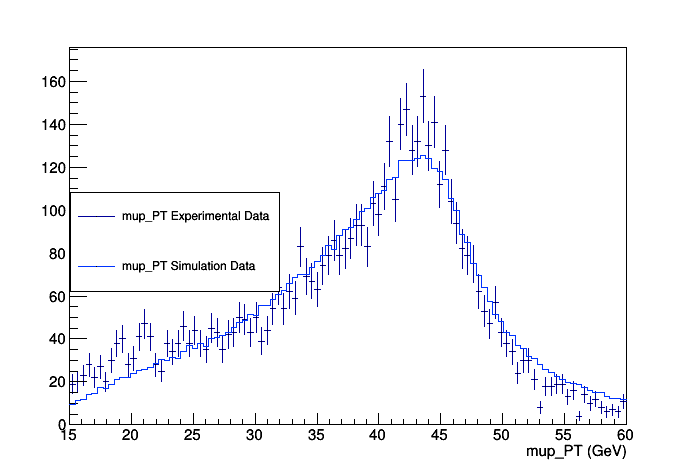
\includegraphics[clip, trim = 0.5cm 0cm 1.7cm 1.3cm, width=0.49\textwidth]{Measurement_mup_PT.png}
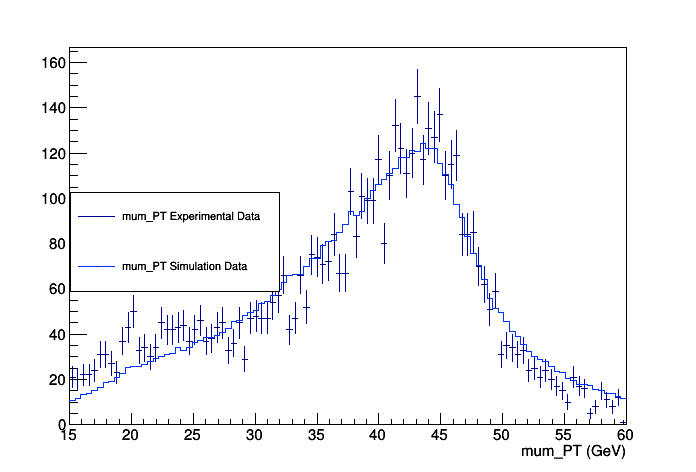
\includegraphics[clip, trim = 0.5cm 0cm 1.7cm 1.3cm, width=0.49\textwidth]{Measurement_mum_PT.png}
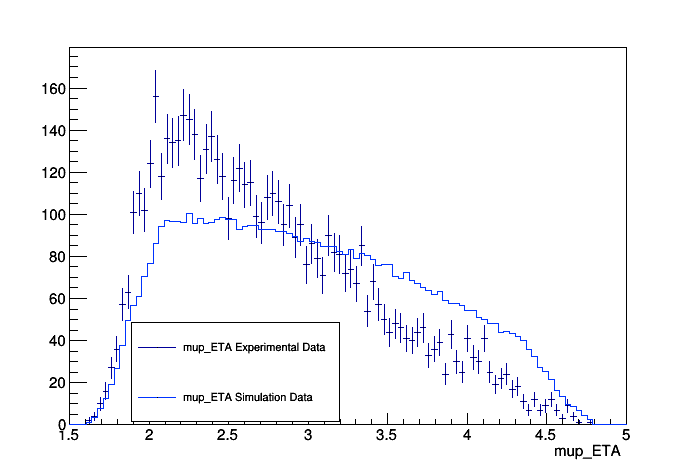
\includegraphics[clip, trim = 0.5cm 0cm 1.7cm 1.3cm, width=0.49\textwidth]{Measurement_mup_ETA.png}
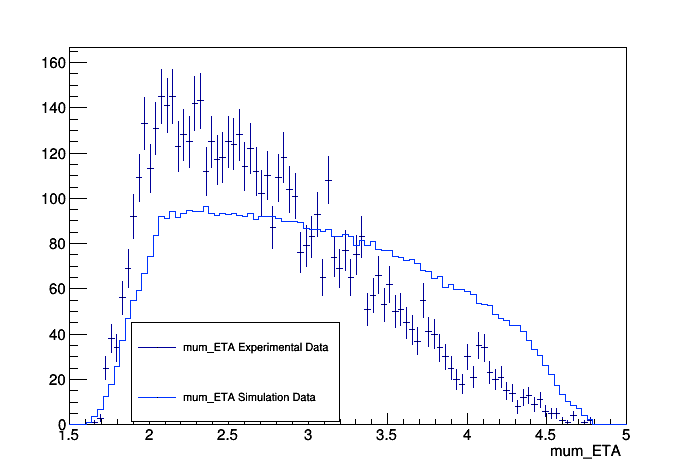
\includegraphics[clip, trim = 0.5cm 0cm 1.7cm 1.3cm, width=0.49\textwidth]{Measurement_mum_ETA.png}
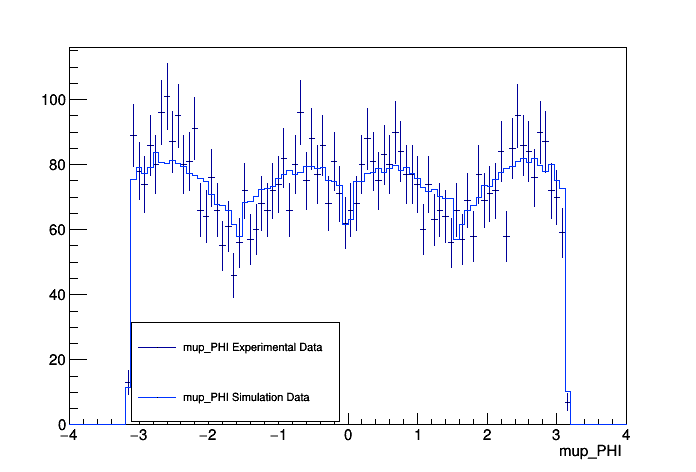
\includegraphics[width=0.49\textwidth]{Measurement_mup_PHI.png}
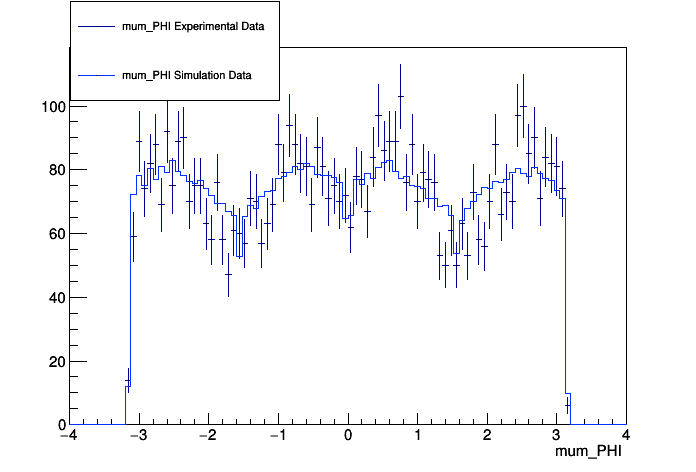
\includegraphics[width=0.49\textwidth]{Measurement_mum_PHI.png}
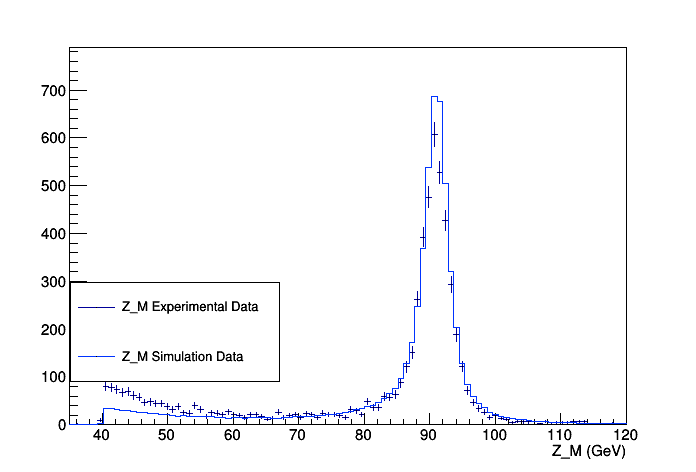
\includegraphics[clip, trim = 0.5cm 0cm 1.7cm 1.3cm, width=0.49\textwidth]{Measurement_Z_M.png}
\vspace{-4mm}
\caption{\small Comparison of $Z$ experimental data with a Monte Carlo simulation with detector reconstruction. Plots are shown for both positive and negative muons, plotting $M_{\mu\mu}$, $p_T$, $\eta$, and $\phi$.}
\label{fig: Z histograms}
\end{figure*}


\bibliography{measurement_report}
\bibliographystyle{h-physrev5}

\end{document}
